% ===============================================================
%  RAPPORT DE PROJET — SMART GRIDS, PROJET 2 « INTÉGRATION DES ENR »
%  Mauges Communauté — ESIEE Paris × Sopra Steria — 2026-2027
% ===============================================================

\documentclass[11pt, a4paper, oneside]{report}

%---------------------------------------------------------------
% ENCODAGE & LANGUE
%---------------------------------------------------------------
\usepackage[utf8]{inputenc}
\usepackage[T1]{fontenc}
\usepackage[french]{babel}
\usepackage{csquotes}
\usepackage[
  backend=biber,
  style=numeric,
  sorting=none
]{biblatex}
\addbibresource{bib.bib}
\addto\captionsfrench{\renewcommand{\listfigurename}{Liste des figures}}
\addto\captionsfrench{\renewcommand{\listtablename}{Liste des tableaux}}

%---------------------------------------------------------------
% MISE EN PAGE & INTERLIGNE
%---------------------------------------------------------------
\usepackage[
  top=2.5cm, bottom=2.5cm,
  left=2.5cm, right=2.5cm,
  headheight=29pt
]{geometry}
\usepackage{setspace}
\setstretch{1.2}

%---------------------------------------------------------------
% TYPOGRAPHIE
%---------------------------------------------------------------
\usepackage{lmodern}
\usepackage{microtype}

%---------------------------------------------------------------
% GRAPHIQUES & COULEURS
%---------------------------------------------------------------
\usepackage{graphicx}
\graphicspath{{figures/}}
\usepackage[dvipsnames, table]{xcolor}
\definecolor{esieeBlue}{RGB}{14, 33, 102}
\definecolor{DarkGray}{RGB}{80, 80, 80}
\definecolor{LightGray}{RGB}{238, 240, 245}
\definecolor{accentOrange}{RGB}{200, 90, 18}

%---------------------------------------------------------------
% EN-TÊTES & PIEDS DE PAGE
%---------------------------------------------------------------
\usepackage{fancyhdr}
\pagestyle{fancy}
\fancyhf{}
\fancyhead[L]{\small\textit{Intégration des ENR à Mauges Communauté}}
\fancyhead[R]{\small\textit{\nouppercase{\leftmark}}}
\fancyfoot[C]{\textcolor{DarkGray}{\thepage}}
\renewcommand{\headrulewidth}{0.4pt}
\renewcommand{\headrule}{\color{esieeBlue}\hrule width\headwidth height\headrulewidth}
\fancypagestyle{plain}{%
  \fancyhf{}
  \fancyfoot[C]{\textcolor{DarkGray}{\thepage}}
  \renewcommand{\headrulewidth}{0pt}
}

%---------------------------------------------------------------
% SECTIONS & TITRES (format compact)
%---------------------------------------------------------------
\usepackage{titlesec}
\titleclass{\chapter}{straight}
\titleformat{\chapter}[hang]
  {\normalfont\huge\bfseries\color{esieeBlue}}
  {\thechapter.}{0.5em}{\huge}
\titlespacing*{\chapter}{0pt}{18pt}{10pt}
\titleformat{\section}
  {\normalfont\Large\bfseries\color{esieeBlue}}
  {\thesection}{1em}{}
\titleformat{\subsection}
  {\normalfont\large\bfseries\color{DarkGray}}
  {\thesubsection}{1em}{}
\titlespacing*{\section}{0pt}{10pt}{4pt}
\titlespacing*{\subsection}{0pt}{8pt}{3pt}

\usepackage[nottoc]{tocbibind}
\usepackage{needspace}

%---------------------------------------------------------------
% LIENS HYPERTEXTES
%---------------------------------------------------------------
\usepackage[
  colorlinks=true,
  linkcolor=esieeBlue,
  citecolor=esieeBlue,
  urlcolor=esieeBlue,
  linktoc=all,
  pdftitle={Intégration des ENR à Mauges Communauté},
  pdfauthor={Noé Quetin, Imran Fagbemi, Konoufo Yacoub Habib Keita}
]{hyperref}
\usepackage{bookmark}
\usepackage{tabularx}

%---------------------------------------------------------------
% MATHÉMATIQUES & UNITÉS
%---------------------------------------------------------------
\usepackage{amsmath, amssymb}
\usepackage{siunitx}
\sisetup{
  locale                = FR,
  output-decimal-marker = {,},
  group-minimum-digits  = 4,
  per-mode              = symbol
}

%---------------------------------------------------------------
% ACRONYMES
%---------------------------------------------------------------
\usepackage[acronym, toc, nonumberlist]{glossaries}
\makeglossaries
\newacronym{enr}{ENR}{Énergies renouvelables}
\newacronym{epci}{EPCI}{Établissement public de coopération intercommunale}
\newacronym{odre}{ODRÉ}{Open Data Réseaux Énergies}
\newacronym{rte}{RTE}{Réseau de transport d'électricité}
\newacronym{insee}{INSEE}{Institut national de la statistique et des études économiques}
\newacronym{sdes}{SDES}{Service des données et études statistiques}
\newacronym{s3renr}{S3REnR}{Schéma régional de raccordement au réseau des énergies renouvelables}
\newacronym{pcaet}{PCAET}{Plan climat-air-énergie territorial}
\newacronym{van}{VAN}{Valeur actuelle nette}
\newacronym{trve}{TRVE}{Tarif réglementé de vente d'électricité}
\newacronym{nrel}{NREL}{National Renewable Energy Laboratory}
\newacronym{cre}{CRE}{Commission de régulation de l'énergie}
\newacronym{dju}{DJU}{Degrés-jours unifiés}
\newacronym{ve}{VE}{Véhicule électrique}
\newacronym{pac}{PAC}{Pompe à chaleur}
\newacronym{utc}{UTC}{Temps universel coordonné}
\newacronym{fc}{FC}{Facteur de charge}
\newacronym{mwc}{MWc}{Mégawatt-crête}
\newacronym{cerema}{Cerema}{Centre d'études et d'expertise sur les risques, l'environnement, la mobilité et l'aménagement}

%---------------------------------------------------------------
% FIGURES & TABLEAUX
%---------------------------------------------------------------
\usepackage{float}
\usepackage{caption}
\captionsetup{font=small, labelfont={bf,color=esieeBlue}, skip=4pt}
\usepackage{booktabs}
\usepackage{array}
\usepackage{tikz}
\usetikzlibrary{arrows.meta, positioning, fit, calc}
\setlength{\textfloatsep}{10pt plus 2pt minus 2pt}
\setlength{\floatsep}{8pt plus 2pt minus 2pt}

%---------------------------------------------------------------
% INFORMATIONS DU DOCUMENT
%---------------------------------------------------------------
\newcommand{\titreRapport}{Intégration des énergies renouvelables à Mauges Communauté}
\newcommand{\sousTitre}{Jusqu'où développer le solaire et l'éolien sans perdre plus de 5\,\% de la production ni saturer le réseau, et avec quelle flexibilité~?}
\newcommand{\typeDocument}{Rapport de projet, réseaux intelligents et stockage de l'énergie}
\newcommand{\anneeUniv}{2026 -- 2027}
\newcommand{\lienSimulateur}{\url{https://quetinn.github.io/simulateur-mauges}}

%===============================================================
\begin{document}
%===============================================================
\pagenumbering{roman}

\begin{titlepage}
  \centering
  \vspace*{0.3cm}
  \begin{minipage}[c]{0.45\textwidth}
    \raggedright
    
\includegraphics[height=2.2cm]{logos/ESIEE.jpg}
  \end{minipage}
  \hfill
  \begin{minipage}[c]{0.45\textwidth}
    \raggedleft
    
\includegraphics[height=2.2cm]{logos/mauges.jpg}
  \end{minipage}

  \vspace{1.5cm}
  \rule{\linewidth}{1.5pt}
  \vspace{0.4cm}

  {\Large\color{esieeBlue}\scshape \typeDocument}\\[0.3cm]
  {\small Projet 2, Intégration des ENR ~|~ ESIEE Paris × Sopra Steria ~|~ Année universitaire \anneeUniv}

  \vspace{1cm}
  \rule{\linewidth}{0.5pt}
  \vspace{1.2cm}

  {\Huge\bfseries\color{esieeBlue} \titreRapport}\\[0.8cm]
  {\large\color{DarkGray} \sousTitre}

  \vspace{1.2cm}
  \rule{\linewidth}{0.5pt}
  \vspace{1.5cm}

  \begin{minipage}[t]{0.55\textwidth}
    \raggedright
    {\large\bfseries\color{esieeBlue} Groupe}\\[0.3cm]
    {\large\bfseries Noé Quetin}\\[0.1cm]
    {\large\bfseries Imran Fagbemi}\\[0.1cm]
    {\large\bfseries Konoufo Yacoub Habib Keita}\\[0.2cm]
    \small 5\textsuperscript{e} année, filière Énergie, ESIEE Paris
  \end{minipage}
  \hfill
  \begin{minipage}[t]{0.4\textwidth}
    \raggedleft
    {\large\bfseries\color{esieeBlue} Encadrants}\\[0.3cm]
    {\large\bfseries Guy Maignant}\\[0.1cm]
    {\large\bfseries Nicolas Cuvelier}\\[0.2cm]
    \small Sopra Steria
  \end{minipage}

  \vfill
  \rule{\linewidth}{1.5pt}\\[0.4cm]
  {\small Simulateur~: \lienSimulateur}\\[0.3cm]
  {\large Soutenance du \textbf{3 novembre 2026}}
\end{titlepage}
\thispagestyle{empty}
\clearpage

\chapter*{Résumé}
\addcontentsline{toc}{chapter}{Résumé}
Mauges Communauté, intercommunalité rurale et industrielle de 123~368 habitants située dans le Maine-et-Loire, produit chaque année avec ses 232~MW d'éoliennes et de panneaux solaires l'équivalent de 42~\% de l'électricité qu'elle consomme. Ce chiffre en volume masque pourtant une autre réalité, puisque la production et la consommation ne coïncident pas dans le temps. Ce rapport cherche jusqu'où le territoire peut développer le solaire et l'éolien sans perdre plus de 5~\% de sa production par écrêtement ni saturer son réseau, et avec quelle flexibilité. Aucune mesure horaire publique n'existant à cette échelle, nous avons reconstruit 43~824 heures de consommation et de production sur les années 2021 à 2025 à partir de données publiques de nature très diverse, électriques, météorologiques, démographiques et foncières. Chaque étape a été confrontée à des contrôles de cohérence. Un moteur de bilan horaire, mis à disposition des élus sous la forme d'un simulateur web, montre que doubler le solaire ne fait gagner que 8 points de couverture tout en faisant perdre 8,2~\% de la production. La batterie demandée par la fiche du projet supprime cet écrêtement mais coûte 186~M€ et ne se rembourse jamais. Nous recommandons plutôt d'augmenter l'éolien de 50~\% et le solaire de 25~\% en chauffant les ballons d'eau chaude à midi. La part de la consommation couverte heure par heure passe alors de 41,6 à 55,4~\%, sans stockage et sous la limite de 5~\% chaque année. Cette trajectoire n'est tenable qu'à condition d'orienter les nouveaux projets vers les postes sources qui disposent encore de capacité d'accueil, selon les capacités financières de raccordement disponibles de la région.

\vspace{0.3cm}
\noindent\textbf{Mots-clés~:} énergies renouvelables~; simulation horaire~; taux de couverture~; écrêtement~; flexibilité~; capacité d'accueil du réseau.

\clearpage

\tableofcontents
\clearpage
\listoffigures
\listoftables
\clearpage
\printglossary[type=\acronymtype, title={Liste des acronymes}, toctitle={Liste des acronymes}]
\clearpage

\pagenumbering{arabic}
\setcounter{page}{1}

% ===============================================================
%  INTRODUCTION (~1 page)
% ===============================================================
\chapter*{Introduction}
\addcontentsline{toc}{chapter}{Introduction}
\markboth{Introduction}{}
\label{chap:intro}

\section*{Un territoire qui produit beaucoup, mais pas au bon moment}

Mauges Communauté est une communauté d'agglomération du sud-ouest du Maine-et-Loire qui regroupe six communes nouvelles et 123~368 habitants sur 1~313~km²~\cite{insee_dossier}. Elle consomme en moyenne 812~GWh d'électricité par an, dont plus d'un tiers pour son industrie~\cite{odre_conso}. Avec 118~MW de solaire répartis sur plus de 5~000 installations et 114~MW d'éolien répartis sur dix parcs~\cite{odre_registre}, le territoire produit chaque année environ 344~GWh, soit 42~\% de sa consommation. Ce chiffre flatteur repose cependant sur une comparaison de volumes annuels. Or l'électricité se consomme au moment où elle est produite, et le surplus solaire d'un midi de juillet ne sert à rien une nuit de janvier. La vraie question est donc de savoir quelle part de la consommation est couverte localement heure par heure, et ce que devient cette part lorsque l'on ajoute des panneaux et des éoliennes.

\section*{Commande et problématique}

La fiche du projet~\cite{fiche_projets} demande d'étudier trois trajectoires de développement. Le scénario A conserve le parc actuel, le scénario B double la puissance solaire et le scénario C la triple tout en augmentant l'éolien de moitié. Deux règles encadrent ces scénarios. L'énergie écrêtée ne doit pas dépasser 5~\% de la production annuelle, et une heure devient une heure de vigilance pour le réseau dès que la production locale dépasse 120~\% de la consommation. Le groupe doit tester une solution de flexibilité, en estimer le coût, développer un simulateur à curseurs et recommander une trajectoire aux élus. Notre travail répond donc à la problématique suivante.

\begin{center}
\begin{minipage}{0.9\textwidth}
\itshape Jusqu'où Mauges Communauté peut-elle développer le solaire et l'éolien sans perdre plus de 5~\% de sa production ni saturer son réseau, et quelle flexibilité le permet au meilleur coût~?
\end{minipage}
\end{center}

\section*{Démarche et organisation du rapport}

Répondre à cette question suppose d'en résoudre quatre autres, qui structurent ce rapport. La première est méthodologique. Comment connaître heure par heure la production et la consommation d'un territoire pour lequel aucune mesure horaire n'est publiée~? Le chapitre~\ref{chap:methode} y répond en détaillant le choix des données, leur traitement et la reconstruction des séries horaires, sans perdre de vue les habitants et les activités qui se cachent derrière les mégawattheures. La deuxième question porte sur les effets physiques des scénarios. Que deviennent le taux de couverture, l'écrêtement et les heures de vigilance quand on augmente le solaire et l'éolien~? La troisième est économique. La batterie demandée par la fiche est-elle une réponse, et à quel coût~? Le chapitre~\ref{chap:resultats} traite ces deux questions. La quatrième est décisionnelle. Quelle trajectoire recommander, et le réseau peut-il l'accueillir~? Le chapitre~\ref{chap:reco} y répond, avant que le chapitre~\ref{chap:discussion} ne discute les limites de l'étude. Tout au long du rapport, nous avons cherché à confronter chaque résultat à un ordre de grandeur indépendant, car un modèle qui ne se remet pas en question produit des chiffres précis mais pas forcément justes.

% ===============================================================
%  CHAPITRE 1 — MÉTHODE (~6 pages)
% ===============================================================
\chapter[Méthode]{Reconstruire heure par heure un territoire sans mesure horaire}
\label{chap:methode}

\section{Démarche d'ensemble et indicateurs}
\label{sec:demarche}

Aucune courbe de charge publique n'existe à la maille d'une intercommunalité. Les gestionnaires de réseau publient en revanche des volumes annuels locaux et des profils horaires régionaux, tandis que d'autres organismes décrivent la météo, la population, le parc automobile ou le foncier. Notre méthode consiste à assembler ces sources pour reconstruire, pour chaque heure de 2021 à 2025, la consommation et la production des Mauges, puis à simuler sur ces séries les scénarios demandés. La figure~\ref{fig:chaine} résume cette chaîne, dont chaque maillon est détaillé dans la suite du chapitre.

\begin{figure}[H]
\centering
\begin{tikzpicture}[
  box/.style={draw=esieeBlue, fill=LightGray, rounded corners=3pt, align=center, font=\footnotesize, minimum height=1.25cm, text width=2.45cm},
  dark/.style={box, fill=esieeBlue, text=white},
  arr/.style={-{Stealth[length=2.5mm]}, thick, color=esieeBlue!70}]
\node[box] (d) {Données publiques\\ électriques, météo,\\ INSEE, réseau, foncier};
\node[box, right=0.45cm of d] (t) {Collecte, traçabilité\\ et harmonisation\\ à l'heure};
\node[box, right=0.45cm of t] (r) {Reconstruction\\ horaire de la\\ consommation et\\ de la production};
\node[box, right=0.45cm of r] (m) {Moteur de bilan\\ horaire, 5 années\\ météo};
\node[dark, right=0.45cm of m] (s) {Indicateurs\\ et simulateur};
\draw[arr] (d) -- (t); \draw[arr] (t) -- (r); \draw[arr] (r) -- (m); \draw[arr] (m) -- (s);
\node[font=\scriptsize\itshape, color=accentOrange, below=0.15cm of t, text width=2.6cm, align=center] {contrôles automatiques};
\node[font=\scriptsize\itshape, color=accentOrange, below=0.15cm of r, text width=2.6cm, align=center] {corrections et\\ recalages};
\node[font=\scriptsize\itshape, color=accentOrange, below=0.15cm of m, text width=2.6cm, align=center] {bilans fermés\\ à chaque heure};
\end{tikzpicture}
\caption{Chaîne de traitement, des données publiques au simulateur}
\label{fig:chaine}
\end{figure}

Les indicateurs sont ceux de la fiche du projet, à savoir l'énergie produite, le taux de couverture, le surplus, le déficit et la pointe d'injection. Leur définition mérite toutefois d'être précisée, car deux \og taux de couverture \fg{} coexistent. Le premier rapporte la production annuelle à la consommation annuelle et ne mesure qu'un volume. Le second, que nous retenons, mesure la part de la consommation réellement satisfaite par la production locale au moment où elle a lieu. En notant $P_h$ la production et $C_h$ la consommation de l'heure $h$, il s'écrit
\begin{equation}
\tau = \frac{\sum_h \min(P_h,\, C_h)}{\sum_h C_h},
\label{eq:couverture}
\end{equation}
la batterie, lorsqu'elle existe, modifiant $P_h$ par ses charges et ses décharges. La fiche ne définit pas précisément l'écrêtement. Nous l'avons interprété comme l'énergie produite au-delà du seuil de vigilance, c'est-à-dire au-delà de $1{,}2\,C_h$, exprimée en pourcentage de la production annuelle. Ce choix relie les deux règles de la fiche et revient à considérer qu'au-delà de 120~\% de la consommation locale, l'injection supplémentaire n'est plus acceptée par le réseau. Enfin, nous exigeons que la limite de 5~\% soit respectée pour chacune des cinq années météo étudiées et pas seulement en moyenne, afin qu'une année ensoleillée ne suffise pas à rendre une trajectoire non conforme.

\section{Comprendre le territoire avant de le modéliser}
\label{sec:territoire}

Avant de calculer, nous avons cherché à comprendre qui consomme dans les Mauges et pourquoi. Cette étape n'est pas décorative. Elle conditionne plusieurs hypothèses du modèle et fournit des ordres de grandeur pour juger de la cohérence des résultats. Les données de l'\gls{insee}~\cite{insee_dossier}, comparées au Maine-et-Loire, à la région et à la France, dessinent un territoire très particulier (figure~\ref{fig:territoire}).

\begin{figure}[H]
\centering
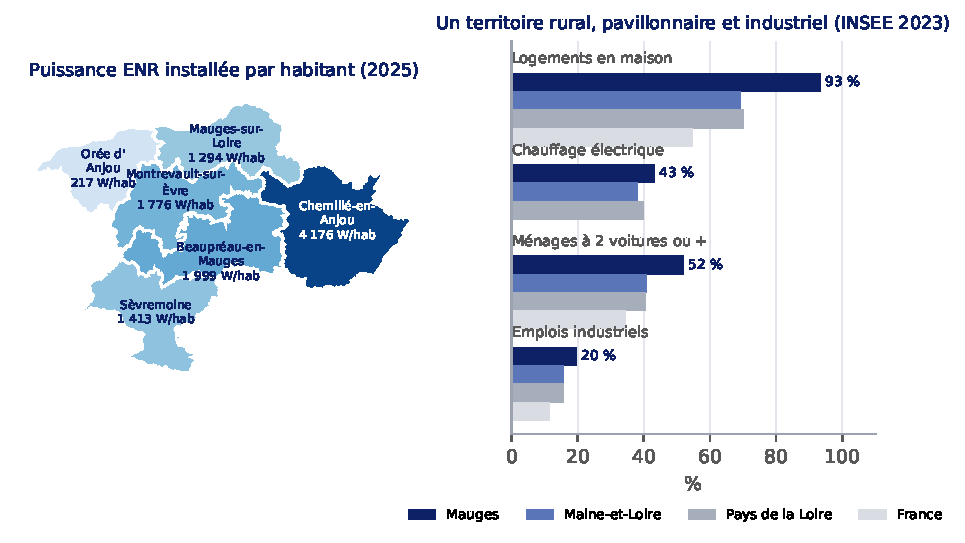
\includegraphics[width=\textwidth]{territoire.pdf}
\caption{Répartition de la puissance renouvelable installée et profil socio-économique des Mauges~\cite{odre_registre, insee_dossier}}
\label{fig:territoire}
\end{figure}

Les Mauges sont d'abord un territoire pavillonnaire. 93~\% des logements sont des maisons, contre 55~\% en France, et 43~\% des résidences principales sont chauffées à l'électricité. Il n'est donc pas surprenant qu'un habitant y consomme 2~455~kWh par an pour son logement en 2023, soit 20~\% de plus que la moyenne française, ni qu'un logement y consomme 5,5~MWh contre 4,1 en moyenne nationale~\cite{enedis_secteur}. C'est ensuite un territoire industriel et agricole, puisque 20~\% des emplois relèvent de l'industrie et 10~\% de l'agriculture, soit presque deux fois et quatre fois la moyenne nationale. L'agroalimentaire représente à lui seul plus du tiers de la consommation industrielle mesurée par Enedis. C'est enfin un territoire où la voiture est indispensable. 52~\% des ménages possèdent au moins deux voitures, contre 35~\% en France, alors que les véhicules électriques ne représentent encore que 2,4~\% du parc en 2025~\cite{sdes_ve}.

Ces constats ont trois conséquences directes sur la modélisation. La forte part de chauffage électrique rend la consommation résidentielle sensible au froid, ce qui justifie de travailler sur plusieurs années météo. Le poids de l'industrie impose de traiter à part les sites raccordés directement au réseau de transport, dont la consommation ne suit pas les saisons (section~\ref{sec:conso}). Enfin, le nombre de ballons d'eau chaude électriques et de véhicules, qui détermine le potentiel des flexibilités étudiées, est estimé à partir de ces données démographiques et non posé arbitrairement.

La carte de la figure~\ref{fig:territoire} soulève une autre question, celle de l'équité territoriale. La puissance renouvelable installée varie de 218~W par habitant à Orée d'Anjou à 4~176~W par habitant à Chemillé-en-Anjou, qui accueille l'essentiel de l'éolien. Une trajectoire de développement ne se juge donc pas seulement sur ses indicateurs globaux. Elle se juge aussi sur la répartition de ses impacts entre les communes, question que nous retrouverons lors de l'étude du réseau.

\section{Choix, collecte et traitement des données}
\label{sec:donnees}

Le tableau~\ref{tab:sources} présente les familles de données mobilisées et l'usage qui en est fait. Nous avons volontairement dépassé les seules données électriques. La météo sert à corriger la production, les données démographiques à dimensionner les usages, les données de réseau à localiser les raccordements et les données foncières à vérifier que la surface ne constitue pas une contrainte.

\begin{table}[H]
\centering
\footnotesize
\caption{Principales sources de données et usage dans l'étude}
\label{tab:sources}
{\renewcommand{\arraystretch}{1.2}
\begin{tabularx}{\textwidth}{@{}>{\raggedright\arraybackslash}p{2.1cm}>{\raggedright\arraybackslash}X>{\raggedright\arraybackslash}p{2.9cm}>{\raggedright\arraybackslash}X@{}}
\toprule
\textbf{Famille} & \textbf{Données} & \textbf{Source} & \textbf{Usage} \\
\midrule
Production & Parc par installation ; production régionale horaire & \gls{odre}~\cite{odre_registre}, \gls{rte}~\cite{rte_eco2mix}, Enedis~\cite{enedis_agregats} & Puissances des scénarios, facteurs de charge \\
Consommation & Volume annuel de l'\gls{epci} par secteur ; profils horaires & \gls{odre}~\cite{odre_conso}, Enedis~\cite{enedis_secteur}, éCO2mix & Courbe de charge locale \\
Météo & Rayonnement, vent, température horaires & Météo-France~\cite{meteofrance} & Corrections de production, \gls{dju} \\
Territoire & Population, logements, chauffage, projections & \gls{insee}~\cite{insee_dossier, insee_omphale} & Ballons, horizon 2035, contrôles \\
Mobilité & Véhicules par commune et type de recharge & \gls{sdes}~\cite{sdes_ve} & Parc de \gls{ve} en 2035 \\
Réseau & Capacité \gls{s3renr} des postes sources ; quote-part & Caparéseau~\cite{capareseau}, DREAL~\cite{dreal_s3renr} & Lieux et coût de raccordement \\
Foncier & Toitures, parkings, zones au sol favorables & \gls{cerema}, IGN~\cite{cerema_pv} & Surface exploitable en solaire \\
Économie & Coût des batteries, tarifs, objectifs locaux & \gls{nrel}~\cite{nrel2025}, \gls{cre}~\cite{cre_trve}, \gls{pcaet}~\cite{pcaet} & \gls{van}, objectifs du territoire \\
\bottomrule
\end{tabularx}}
\end{table}

Les données ont été collectées par les interfaces de programmation d'ODRÉ et d'Enedis ou par export direct, soit 46 téléchargements. Chacun est consigné dans un manifeste qui conserve l'adresse exacte de la requête, la date et l'empreinte du fichier, de sorte que toute la chaîne peut être rejouée. Les séries ont ensuite été harmonisées. Les données au pas de 30~minutes ont été ramenées à l'heure, toutes les dates exprimées en \gls{utc} pour éviter les doublons du changement d'heure, et les unités converties en MW et MWh. Les trous de deux heures au plus ont été comblés par interpolation linéaire et signalés, ce qui concerne 2,4~\% des heures, principalement en 2024 et 2025. Les trous plus longs ont été laissés vides. Un script de contrôle vérifie enfin à chaque relance les bilans, les bornes physiques et l'absence de valeurs aberrantes.

Ces contrôles ont permis de détecter plusieurs incohérences avant qu'elles ne contaminent les résultats. Enedis indique par exemple pour 2022 des degrés-jours inférieurs de 41~\% à ceux de 2021, alors que nos degrés-jours recalculés à partir de la station Météo-France de Saint-Florent-le-Vieil ne baissent que de 16 à 22~\% selon la convention retenue. Pour toutes les autres années, nos calculs encadrent pourtant ceux d'Enedis. Nous avons donc écarté la valeur 2022 publiée. De même, en 2024, ODRÉ classe 130~GWh en \og non affecté \fg{} et retire autant de l'industrie, ce qui nous a conduits à calculer la répartition sectorielle sur la période 2021-2023.

\section{Reconstruire la consommation horaire}
\label{sec:conso}

La consommation horaire des Mauges est obtenue en répartissant le volume annuel mesuré selon une forme horaire régionale. L'hypothèse sous-jacente est qu'à l'intérieur d'un même secteur, un logement ou une usine des Mauges consomme au même rythme que son homologue régional. Le volume local capte donc le poids propre du territoire, tandis que la forme régionale apporte la météo de l'année et les cycles journaliers et hebdomadaires. Deux variantes ont été construites. La méthode S applique à chaque secteur le profil Enedis correspondant, disponible pour 2024 et 2025. La méthode R utilise la consommation régionale publiée par éCO2mix, disponible sur les cinq années. La figure~\ref{fig:conso} montre qu'elles sont très proches. Sur 2024, leur corrélation horaire atteint 0,97, la pointe diffère de 2,8~\% et l'écrêtement du scénario B de 0,2 point seulement. Nous avons donc retenu la méthode R pour les cinq années.

\begin{figure}[H]
\centering
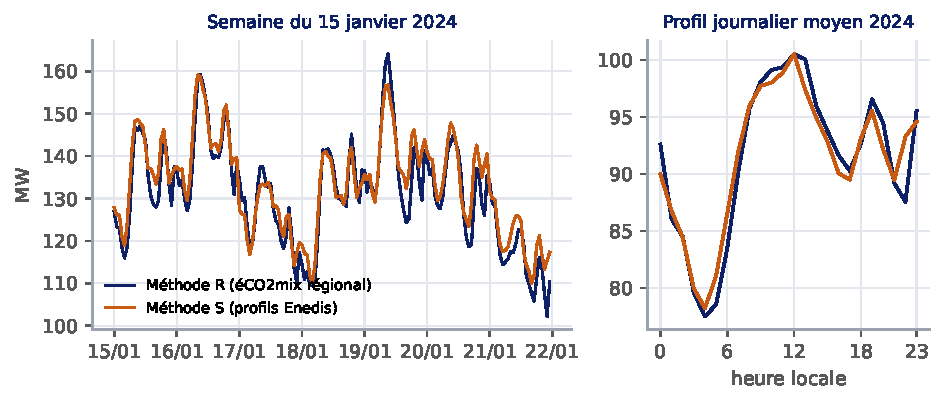
\includegraphics[width=\textwidth]{conso_methodes.pdf}
\caption{Comparaison des deux méthodes de reconstruction de la consommation (2024)}
\label{fig:conso}
\end{figure}

Deux corrections complètent cette reconstruction. La consommation de 2025 n'étant pas encore publiée, nous l'avons estimée en appliquant au volume de 2024 l'évolution de la consommation régionale entre 2024 et 2025, et signalée comme telle. Surtout, l'écart entre la consommation totale publiée par ODRÉ et la somme des consommations communales d'Enedis représente chaque année entre 14,5 et 16,6~\% du total. Cet écart correspond aux sites raccordés directement au réseau de transport, essentiellement industriels, ce que confirme le fait qu'il se retrouve presque entièrement dans le secteur industriel. Or la consommation nationale de ces clients ne présente pratiquement aucune saisonnalité, avec un rapport hiver sur été de 0,96 contre 1,47 pour la consommation totale. Appliquer à cette part le profil régional, très marqué par le chauffage, aurait donc surestimé les pointes d'hiver. Nous l'avons modélisée par un profil plat, ce qui réduit la pointe de soutirage d'environ 8~\%.

\section{Reconstruire la production horaire}
\label{sec:prod}

La production horaire est obtenue en multipliant la puissance installée dans les Mauges par le facteur de charge régional de chaque heure, publié par éCO2mix pour le solaire et l'éolien. Les autres filières, bioénergie et hydraulique, représentent moins de 2~\% de la production et sont considérées comme constantes. Le même parc, celui du 31 décembre 2025, est appliqué aux cinq années afin de ne faire varier que la météo. Cette construction simple a cependant révélé deux biais qu'il a fallu corriger.

Le premier vient d'éCO2mix lui-même. Le facteur de charge publié est le rapport entre la production et une capacité installée qui n'est mise à jour que par paliers. Entre deux mises à jour, le parc réel continue de croître alors que le dénominateur reste figé, si bien que le facteur de charge dérive à la hausse puis chute brutalement. Ainsi, la capacité solaire régionale reste fixée à 1~212~MW de décembre 2023 à novembre 2024 avant de bondir à 1~642~MW (figure~\ref{fig:capacite}). Nous avons reconstruit une capacité lissée par interpolation linéaire entre les paliers, en considérant que chaque palier publié correspond au parc réel à sa date. Le facteur de charge solaire de 2024 passe alors de 13,8 à 11,6~\%, ce qui fait de 2024 l'année la moins ensoleillée de la période. Ce résultat est cohérent avec le rayonnement mesuré à Beaucouzé, qui est lui aussi le plus faible en 2024.

\begin{figure}[H]
\centering
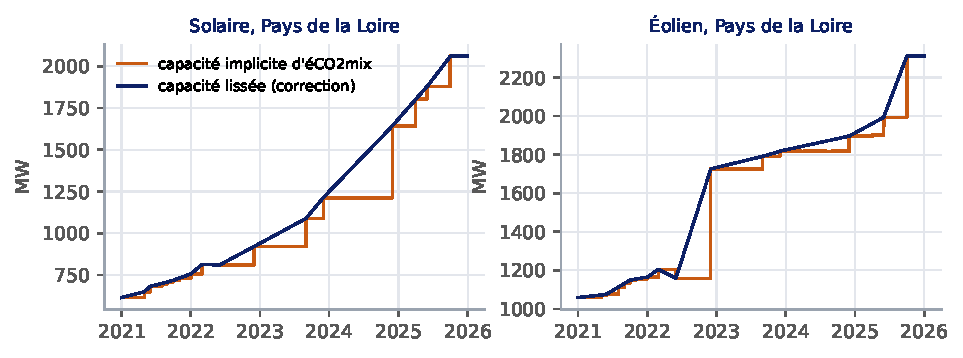
\includegraphics[width=\textwidth]{capacite_eco2mix.pdf}
\caption{Capacité installée implicite d'éCO2mix et capacité lissée retenue}
\label{fig:capacite}
\end{figure}

Le second biais concerne l'éolien. Depuis la mise en service du parc en mer de Saint-Nazaire fin 2022, le profil régional mêle production en mer et production terrestre, alors que les Mauges n'ont que des éoliennes terrestres. À vent égal mesuré à Cholet, le facteur de charge régional augmente de 6 à 17~\% après cette date. Nous avons donc corrigé le niveau annuel de l'éolien à vent égal, année par année. Pour vérifier que la forme horaire n'était pas elle aussi biaisée, nous l'avons remplacée en 2024 et 2025 par celle de la production éolienne d'Enedis, qui ne concerne que des parcs terrestres. Le taux de couverture varie de moins d'un point, ce qui nous a conduits à conserver la forme éCO2mix, seule disponible sur toute la période.

Enfin, les productions simulées ont été recalées sur la production réellement injectée par les installations des Mauges, issue du registre national. Les coefficients obtenus valent 0,900 pour le solaire et 0,859 pour l'éolien, les installations locales produisant un peu moins que la moyenne régionale. Cette étape répond aussi à une question posée par la fiche, qui impose 15~\% de pertes photovoltaïques. Notre production étant calée sur des mesures réelles, ces pertes y sont déjà incluses, et les appliquer une seconde fois reviendrait à les compter deux fois.

\section{Moteur de simulation, hypothèses et validation}
\label{sec:moteur}

Le moteur calcule pour chaque heure le bilan entre production et consommation, puis les indicateurs de la section~\ref{sec:demarche}. La batterie de la fiche a une puissance égale à la puissance solaire du scénario, une durée de deux heures et un rendement aller-retour de 90~\%. Deux pilotages ont été comparés. Le premier stocke tout surplus dès que la production dépasse la consommation, ce qui maximise la couverture mais remplit souvent la batterie avant le pic de midi. Le second ne stocke que l'énergie qui dépasse le seuil de 120~\%, afin de garder sa capacité pour éviter l'écrêtement. Trois autres leviers ont été modélisés, à savoir le déplacement vers la mi-journée de la chauffe des ballons d'eau chaude, le pilotage de la recharge des \gls{ve} et un plafond d'injection des installations solaires. Un horizon 2035 intègre enfin l'électrification des usages à partir des hypothèses des fiches des projets 1 et 3 et des projections de l'\gls{insee}, avec 25~\% des logements équipés d'une \gls{pac} et 40~\% de véhicules électriques~\cite{fiche_projets, insee_omphale, rte_bp2025}. L'ensemble des hypothèses et de leurs sources figure en annexe~\ref{annexe:hypotheses}.

Le volet économique repose sur la \gls{van} sur 15 ans, actualisée à 4~\% selon le taux retenu par \gls{rte}~\cite{rte_fe2050}.
\begin{equation}
\mathrm{VAN} = -I + \sum_{t=1}^{15} \frac{G - C_{\mathrm{OM}}}{(1+0{,}04)^{t}},
\label{eq:van}
\end{equation}
où $I$ est l'investissement, $G$ le gain annuel et $C_{\mathrm{OM}}$ le coût annuel d'exploitation. Les coûts proviennent des projections du \gls{nrel} pour 2025, soit 395~€ par kWh de capacité et 49~€ par kW et par an d'exploitation~\cite{nrel2025, bce}. Le gain correspond à l'électricité qui n'est plus achetée au réseau, valorisée au tarif réglementé de 0,194~€/kWh~\cite{cre_trve}, diminuée du surplus qui n'est plus vendu à 0,02~€/kWh~\cite{cre_surplus}.

Les résultats sont donnés en moyenne sur 2021-2025 avec la fourchette des cinq années. L'année 2022, la plus proche de la moyenne sur l'ensemble des indicateurs, sert d'année type pour les représentations heure par heure. Un modèle peut tourner sans erreur et rester faux, c'est pourquoi nous avons vérifié le moteur par des propriétés physiques. À chaque heure, la consommation doit se répartir exactement entre production locale, décharge de la batterie et achats au réseau, et la production entre consommation directe, charge et export, faute de quoi le calcul s'arrête. Le scénario A sert aussi de témoin, puisque sa couverture horaire doit rester proche de sa couverture en volume (section~\ref{sec:actuel}), et les principaux ordres de grandeur se recalculent à la main (annexe~\ref{annexe:calculs}). Le simulateur, accessible à l'adresse \lienSimulateur, repose sur ce même moteur. Il permet de faire varier chaque hypothèse et propose une vue destinée aux élus, une vue de démonstration et une vue experte (figure~\ref{fig:simulateur}).

\begin{figure}[H]
\centering
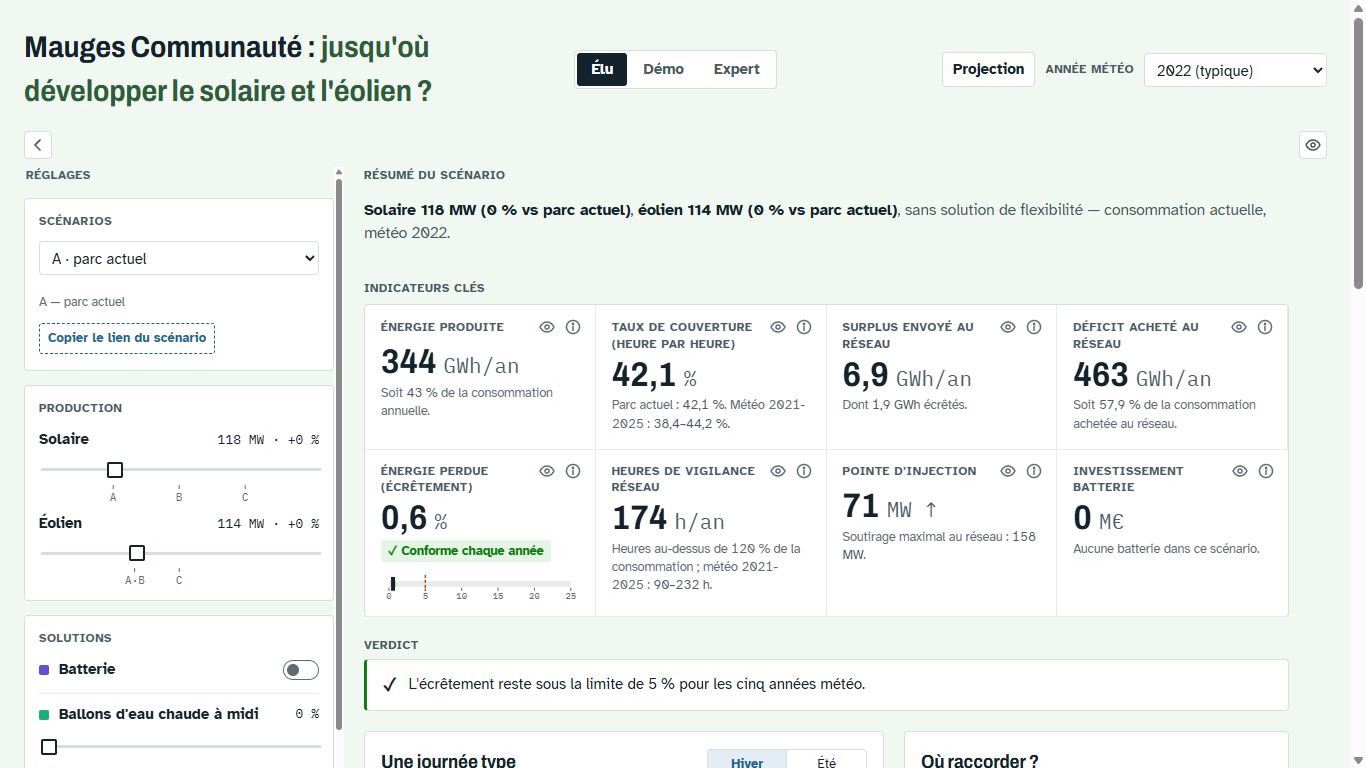
\includegraphics[width=0.82\textwidth]{simulateur_elu.png}
\caption{Vue Élu du simulateur, scénario A, année météo 2022}
\label{fig:simulateur}
\end{figure}

% ===============================================================
%  CHAPITRE 2 — RÉSULTATS (~4 pages)
% ===============================================================
\chapter[Résultats]{Ce que montre la simulation}
\label{chap:resultats}

\section{La situation actuelle}
\label{sec:actuel}

Avec le parc actuel, la production locale couvre 41,6~\% de la consommation heure par heure en moyenne, entre 38,4~\% et 44,2~\% selon l'année météo. Ce chiffre est très proche des 42~\% obtenus en volume, et cette proximité est en elle-même un résultat. Elle signifie qu'aujourd'hui la production ne dépasse presque jamais la consommation, puisque le surplus envoyé hors du territoire ne représente que 7~GWh par an, soit 2~\% de la production. Le parc actuel est donc loin de toute saturation. Il reste néanmoins 58,5~\% de l'électricité à acheter au réseau, et jusqu'à 68,5~\% en hiver.

\begin{figure}[H]
\centering
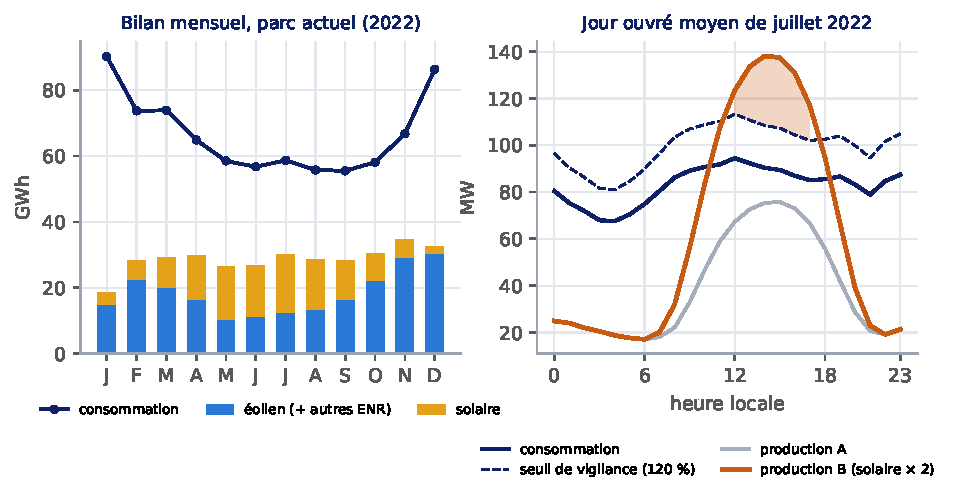
\includegraphics[width=\textwidth]{saisonnalite.pdf}
\caption{Bilan mensuel du parc actuel et jour ouvré moyen de juillet pour les scénarios A et B (2022)}
\label{fig:saison}
\end{figure}

La figure~\ref{fig:saison} explique cette situation. La consommation est maximale en hiver, avec près de 90~GWh en janvier contre 56~GWh en été, sous l'effet du chauffage électrique identifié à la section~\ref{sec:territoire}. L'éolien, qui fournit près des deux tiers de la production, suit heureusement cette saisonnalité. Le solaire produit au contraire l'essentiel de son énergie d'avril à septembre, et toujours autour de midi. C'est cette concentration temporelle qui va limiter son développement.

\section{Les scénarios B et C}
\label{sec:bc}

Le tableau~\ref{tab:scenarios} présente les indicateurs de la fiche pour les trois scénarios. Doubler le solaire augmente la production de 35~\%, mais le taux de couverture ne gagne que 8 points, de 41,6 à 49,5~\%. L'écart entre la couverture en volume et la couverture horaire, quasi nul aujourd'hui, se creuse fortement. Il atteint 7 points en B et 24 points en C, où la production annuelle couvre pourtant 86~\% de la consommation.

\begin{table}[H]
\centering
\footnotesize
\caption{Indicateurs de la fiche pour les trois scénarios, moyenne 2021-2025 et fourchette des cinq années}
\label{tab:scenarios}
{\renewcommand{\arraystretch}{1.2}
\begin{tabularx}{\textwidth}{@{}l>{\centering\arraybackslash}X>{\centering\arraybackslash}X>{\centering\arraybackslash}X@{}}
\toprule
\textbf{Indicateur} & \textbf{A, parc actuel} & \textbf{B, solaire × 2} & \textbf{C, solaire × 3, éolien × 1,5} \\
\midrule
Énergie produite (GWh/an) & 344 & 465 & 694 \\
Production / consommation & 42~\% & 57~\% & 86~\% \\
Taux de couverture horaire & 41,6~\% [38,4 ; 44,2] & 49,5~\% [46,6 ; 51,9] & 61,7~\% [58,8 ; 64,0] \\
Surplus envoyé au réseau (GWh/an) & 7 & 63 & 193 \\
Déficit acheté au réseau (GWh/an) & 475 & 411 & 311 \\
Énergie écrêtée & 0,6~\% [0,2 ; 0,9] & \textcolor{accentOrange}{8,2~\% [5,9 ; 10,3]} & \textcolor{accentOrange}{21,0~\% [18,1 ; 23,7]} \\
Heures de vigilance (h/an) & 165 & 1~236 & 2~363 \\
Pointe d'injection (MW) & 65 & 134 & 241 \\
\bottomrule
\end{tabularx}}
\end{table}

Le jour moyen de juillet de la figure~\ref{fig:saison} montre le mécanisme. En B, la production de midi dépasse le seuil de 120~\% de la consommation pendant environ six heures, et l'énergie située au-dessus de ce seuil doit être écrêtée. L'écrêtement atteint ainsi 8,2~\% de la production en moyenne et dépasse la limite de 5~\% chacune des cinq années, y compris en 2024, la moins ensoleillée. Le scénario C la dépasse largement avec 21~\%. Les heures de vigilance passent de 165 à plus de 2~300 par an, soit plus d'une heure sur quatre. En C, la pointe d'injection de 241~MW dépasse même la pointe de consommation du territoire, qui est de 166~MW. Le réseau local devrait alors évacuer vers l'extérieur une puissance supérieure à tout ce que le territoire peut consommer.

Ces ordres de grandeur sont cohérents entre eux. L'énergie écrêtée en B représente 8,2~\% de 465~GWh, soit environ 38~GWh. Elle est comprise dans les 63~GWh de surplus, qui regroupent toute l'énergie produite au-delà de la consommation, si bien que seuls 25~GWh environ seraient réellement exportés hors du territoire. Le bilan se referme aussi par la consommation, puisque l'énergie couverte localement et le déficit acheté au réseau redonnent bien les 812~GWh consommés. Ni le scénario B ni le scénario C ne respectent donc la règle de la fiche sans flexibilité.

\section{La solution testée, la batterie de la fiche}
\label{sec:batterie}

La fiche impose de tester une batterie dont la capacité correspond à deux heures de la puissance solaire, soit 471~MWh pour le scénario B et 706~MWh pour le scénario C. Techniquement, la batterie remplit son rôle en B. Avec le pilotage qui ne stocke que les excès, l'écrêtement tombe à 0,4~\% en moyenne et ne dépasse jamais 0,8~\%, tandis que la couverture monte à 53,5~\%. En C en revanche, même cette batterie ne suffit pas, puisque l'écrêtement reste de 6,2~\% en moyenne et atteint 8,9~\% la pire année. La figure~\ref{fig:batterie} montre qu'en B, environ 140~MWh suffisent pour respecter la limite de 5~\% chaque année, soit trois fois moins que la taille imposée par la fiche. En C, même 1~060~MWh laissent encore 7,5~\% d'écrêtement la pire année. Elle confirme aussi qu'à taille égale, le pilotage qui réserve la batterie aux excès écrête nettement moins que celui qui stocke tout surplus.

\begin{figure}[H]
\centering
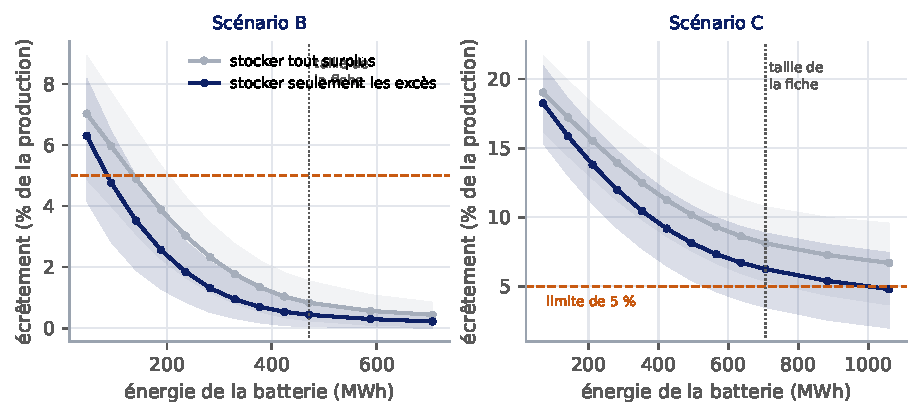
\includegraphics[width=\textwidth]{batterie_taille.pdf}
\caption{Écrêtement en fonction de la taille de la batterie, moyenne et fourchette 2021-2025}
\label{fig:batterie}
\end{figure}

Le coût relatif de cette solution est en revanche rédhibitoire. La batterie du scénario B représente un investissement de 186~M€ et un coût d'exploitation de 11,5~M€ par an. Elle ne fait économiser que 6,4 à 9,7~M€ d'achats d'électricité par an selon le pilotage. Son coût d'exploitation dépasse donc à lui seul le gain qu'elle procure, et sa \gls{van} sur 15 ans vaut entre $-207$ et $-243$~M€. Rapporté au gain de couverture, chaque point supplémentaire coûte environ 46~M€ d'investissement. Une batterie plus petite ne change pas la conclusion. La plus petite capacité qui respecte la limite chaque année, environ 140~MWh, coûterait 56~M€ et rapporterait 3,9~M€ par an pour 3,5~M€ d'exploitation, soit une \gls{van} de $-51$~M€. Nous nous sommes demandé si ce verdict tenait à nos hypothèses de prix. Le tableau~\ref{tab:eco} montre qu'aucune combinaison raisonnable ne rend la batterie rentable, même avec un coût de 250~€/kWh. Valoriser l'électricité évitée au tarif réglementé est d'ailleurs favorable à la batterie, car les industriels, qui consomment plus du tiers de l'électricité du territoire, paient leur électricité bien moins cher que ce tarif résidentiel. Au prix de gros, la \gls{van} se dégrade jusqu'à $-292$~M€. En C, la batterie coûterait 279~M€ sans même rendre le scénario conforme.

\begin{table}[H]
\centering
\footnotesize
\caption{Valeur actuelle nette de la batterie du scénario B (471~MWh) selon les hypothèses économiques}
\label{tab:eco}
{\renewcommand{\arraystretch}{1.2}
\begin{tabularx}{\textwidth}{@{}>{\raggedright\arraybackslash}X cccc@{}}
\toprule
\textbf{Hypothèses} & \textbf{Investissement} & \textbf{Gain annuel} & \textbf{VAN, tout surplus} & \textbf{VAN, excès seuls} \\
\midrule
Base, tarif réglementé 0,194~€/kWh & 186~M€ & 9,7 / 6,4~M€ & $-207$~M€ & $-243$~M€ \\
Prix de gros 0,061~€/kWh & 186~M€ & 2,7 / 2,0~M€ & $-284$~M€ & $-292$~M€ \\
Batterie à 250~€/kWh & 118~M€ & 9,7 / 6,4~M€ & $-91$~M€ & $-128$~M€ \\
Batterie à 500~€/kWh & 235~M€ & 9,7 / 6,4~M€ & $-290$~M€ & $-326$~M€ \\
Hypothèses du projet 6 (10 ans, 5~\%) & 235~M€ & 8,8 / 6,6~M€ & $-167$~M€ & $-184$~M€ \\
\bottomrule
\end{tabularx}}
\end{table}

\section{Les autres leviers et les trajectoires possibles}
\label{sec:leviers}

La batterie n'étant pas une réponse économiquement défendable, nous avons étudié les autres leviers modélisés dans le simulateur. Le plus efficace est le déplacement de la chauffe des ballons d'eau chaude. Faute de statistique locale sur l'eau chaude, nous avons supposé qu'environ la moitié des résidences principales recensées par l'\gls{insee}, soit 26~000 logements, dispose d'un ballon électrique, ce qui correspond à l'ordre de grandeur national d'une quinzaine de millions de chauffe-eau pour 30 millions de résidences principales~\cite{construction21}. Ces ballons représentent 58~MW de puissance et 26~GWh par an. Les chauffer entre 10~h et 17~h plutôt que la nuit permet d'absorber une partie du surplus solaire sans aucun équipement lourd, et la réforme des heures creuses engagée par la \gls{cre}, qui place des heures creuses l'après-midi en été, va déjà dans ce sens~\cite{cre_hphc}. Dans le scénario finalement recommandé, ce levier fait passer l'écrêtement de 4,0 à 3,2~\% et celui de la pire année de 5,0 à 4,1~\%, ce qui fait sortir la trajectoire de la zone limite. Ce levier concerne cependant directement les ménages, et sa mise en œuvre suppose un signal tarifaire ou un pilotage accepté par les habitants. Le pilotage de la recharge des \gls{ve} n'a d'effet qu'à l'horizon 2035, lorsque le parc atteindrait environ 30~600 véhicules. Même en déplaçant à midi l'ensemble des recharges pilotables, le gain de couverture ne dépasse pas 0,4 point. Le plafond d'injection, enfin, réduit l'écrêtement en limitant la puissance des onduleurs, mais il perd l'énergie au lieu de la déplacer.

Pour savoir jusqu'où aller sans stockage, nous avons simulé 360 combinaisons de puissances solaire et éolienne, de leviers et d'horizons. La figure~\ref{fig:trajectoires} présente le cas avec les ballons pilotés. Elle met en évidence une concurrence entre l'éolien et le solaire. Plus on ajoute d'éolien, moins il reste de place pour le solaire sous la limite de 5~\%. Avec 75~\% d'éolien en plus, le parc solaire actuel dépasse déjà la limite certaines années. Le taux de couverture maximal atteignable sans stockage se situe autour de 55 à 57~\%, obtenu avec 50~\% d'éolien en plus et entre 25 et 40~\% de solaire en plus.

\begin{figure}[H]
\centering
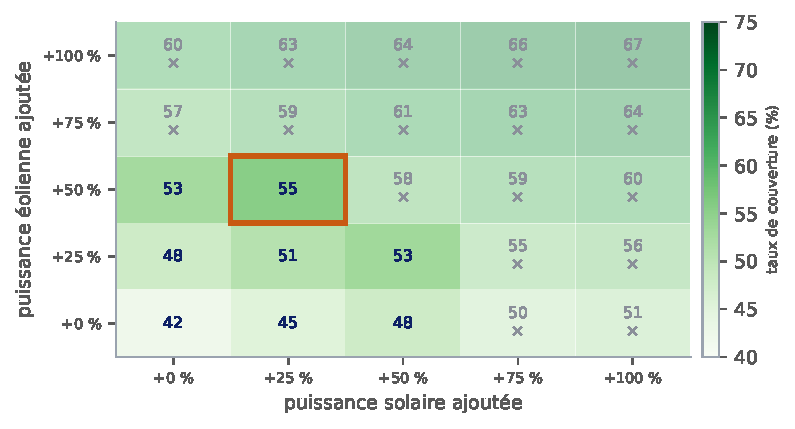
\includegraphics[width=0.8\textwidth]{trajectoires.pdf}
\caption{Taux de couverture moyen selon la puissance ajoutée, avec les ballons pilotés. Les croix signalent un écrêtement supérieur à 5~\% au moins une année, le cadre orange le scénario recommandé}
\label{fig:trajectoires}
\end{figure}

Ces conclusions résistent-elles aux incertitudes du modèle~? Une analyse de sensibilité, qui fait varier une à une les principales hypothèses entre une valeur basse et une valeur haute, montre que l'année météo reste le facteur le plus influent, devant la taille et le pilotage de la batterie. La forme du profil de consommation et le rendement de la batterie n'ont en revanche qu'un effet marginal. Les conclusions ne reposent donc pas sur les choix de reconstruction les plus incertains. À l'horizon 2035 enfin, l'électrification des usages porterait la consommation de 812 à 904~GWh. La couverture du parc actuel baisserait de 41,6 à 37,4~\%, mais l'écrêtement diminuerait aussi, puisque la consommation supplémentaire absorberait une partie des surplus.

% ===============================================================
%  CHAPITRE 3 — RECOMMANDATION ET RÉSEAU (~2 pages)
% ===============================================================
\chapter[Recommandation et réseau]{Recommandation et capacité d'accueil du réseau}
\label{chap:reco}

\section{La trajectoire recommandée}
\label{sec:trajectoire}

Nous recommandons d'augmenter la puissance éolienne de 50~\% et la puissance solaire de 25~\%, en déplaçant la chauffe des ballons d'eau chaude vers la mi-journée et sans investir dans le stockage. Cela représente 57~MW d'éolien et 29~MW de solaire supplémentaires. Le tableau~\ref{tab:reco} compare cette trajectoire à la situation actuelle.

\begin{table}[H]
\centering
\footnotesize
\caption{Trajectoire recommandée comparée au parc actuel, moyenne 2021-2025}
\label{tab:reco}
{\renewcommand{\arraystretch}{1.2}
\begin{tabularx}{0.85\textwidth}{@{}>{\raggedright\arraybackslash}X cc@{}}
\toprule
\textbf{Indicateur} & \textbf{Aujourd'hui} & \textbf{Recommandé} \\
\midrule
Puissance solaire / éolienne & 118 / 114~MW & 147 / 172~MW \\
Énergie produite & 344~GWh/an & 480~GWh/an \\
Taux de couverture horaire & 41,6~\% & \textbf{55,4~\%} [51,5 ; 58,4] \\
Énergie écrêtée (pire année) & 0,6~\% (0,9~\%) & 3,2~\% (4,1~\%) \\
Électricité achetée au réseau & 475~GWh (58,5~\%) & 363~GWh (44,7~\%) \\
Électricité achetée en hiver & 68,5~\% & 56,8~\% \\
Pointe d'injection & 65~MW & 112~MW \\
Investissement de stockage & aucun & aucun \\
\bottomrule
\end{tabularx}}
\end{table}

Ce choix ne correspond pas au maximum de la figure~\ref{fig:trajectoires}. Il serait possible d'aller jusqu'à environ 40~\% de solaire supplémentaire, mais l'écrêtement de la pire année serait alors au contact de la limite et une année plus ensoleillée que celles de la période suffirait à la dépasser. Avec 25~\% de solaire, la pire année reste à 4,1~\%, ce qui laisse une marge face à l'incertitude météorologique. La comparaison avec la batterie est éloquente. La trajectoire recommandée couvre davantage la consommation que le scénario B équipé de sa batterie, soit 55,4 contre 53,5~\%, sans les 186~M€ d'investissement. Elle reste conforme à l'horizon 2035, avec 50,6~\% de couverture et 2,4~\% d'écrêtement. L'éolien est plus utile que le solaire parce qu'il produit surtout en hiver et la nuit, précisément quand la consommation est la plus forte et le solaire absent. La part d'électricité achetée en hiver baisse ainsi de 12 points.

La baisse des achats au réseau, de 112~GWh par an, représente environ 22~M€ par an au tarif réglementé. Ce montant doit être lu comme une borne haute. Les industriels paient leur électricité nettement moins cher, et au prix de gros l'économie serait plutôt de l'ordre de 7~M€. Ce gain ne se traduirait pas non plus mécaniquement sur la facture des ménages, puisque l'électricité produite localement est vendue par ses producteurs sur le marché. Le bénéfice pour le territoire tient surtout à une moindre dépendance au réseau national, en particulier en hiver.

Deux points de vigilance relèvent davantage de la décision politique que de la simulation. Le premier concerne l'objectif du \gls{pcaet}, qui vise 175~GWh de production solaire en 2030~\cite{pcaet}. Notre trajectoire n'en produit que 151~GWh. Atteindre cet objectif demanderait environ 45~\% de solaire en plus, ce qui reste possible sous la limite de 5~\% à condition de limiter l'éolien à 25~\% supplémentaires, avec une couverture ramenée à 52,6~\%. Les élus doivent donc arbitrer entre l'objectif solaire affiché et le meilleur taux de couverture. Le second concerne l'acceptabilité de l'éolien. Le \gls{pcaet} ne fixe pas d'objectif éolien et le territoire a engagé en 2023 une concertation sur les zones d'accélération des énergies renouvelables. Les 57~MW d'éolien supplémentaires représentent cinq à six parcs comparables à ceux d'aujourd'hui. Compte tenu de la concentration actuelle à Chemillé-en-Anjou (section~\ref{sec:territoire}), leur localisation pose une question d'équité entre les communes autant qu'une question technique.

Le foncier, en revanche, n'est pas une contrainte. D'après les données du \gls{cerema} et de l'IGN~\cite{cerema_pv}, le potentiel théorique des toitures atteint environ 2~750~\gls{mwc}. En ne mobilisant que 10~\% de ce potentiel, les 525 parkings de plus de 500~m² et les 112~ha de zones au sol jugées favorables, environ 590~MWc seraient disponibles, soit vingt fois les 29~MWc nécessaires. Les toitures suffiraient même au scénario C.

\section{La capacité d'accueil du réseau}
\label{sec:reseau}

L'énergie produite dans les Mauges rejoint le réseau de transport par des postes sources, dont la capacité d'accueil réservée aux énergies renouvelables est fixée par le \gls{s3renr}. Nous avons collecté sur Caparéseau~\cite{capareseau}, pour les neuf postes qui desservent le territoire, la capacité réservée, la capacité restante et les projets en file d'attente. Faute de connaître l'emplacement des futurs projets, nous avons supposé que la puissance ajoutée se répartit comme le parc existant. Un poste qui porte aujourd'hui 20~\% de l'éolien reçoit ainsi 20~\% de l'éolien ajouté. La figure~\ref{fig:postes} compare cet ajout à la capacité restante de chaque poste.

\begin{figure}[H]
\centering
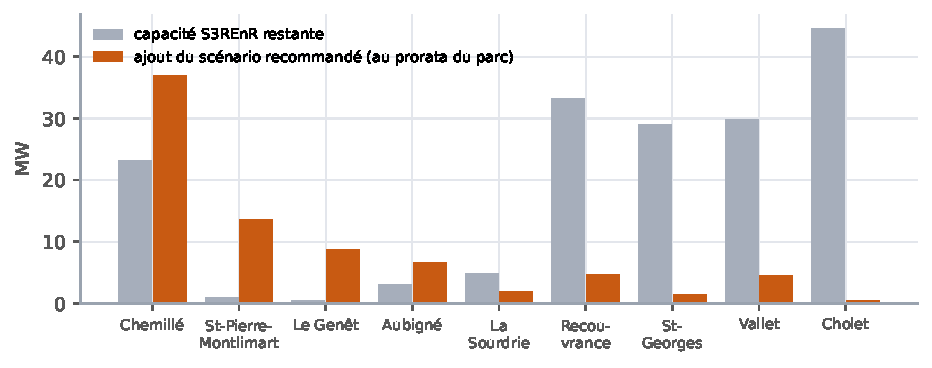
\includegraphics[width=\textwidth]{postes.pdf}
\caption{Capacité S3REnR restante et puissance ajoutée par poste source dans le scénario recommandé~\cite{capareseau, odre_registre}}
\label{fig:postes}
\end{figure}

Étendu de cette manière, le scénario recommandé saturerait quatre postes. Chemillé serait dépassé de 14~MW, Saint-Pierre-Montlimart de 13~MW, Le Genêt de 8~MW et Aubigné de 4~MW. Le scénario B saturerait déjà trois postes et le scénario C six sur neuf, avec un dépassement de 53~MW à Chemillé. Pourtant, la capacité restante totale de 169~MW est largement suffisante. Elle est simplement mal répartie, puisque Recouvrance, Vallet, Saint-Georges et Cholet disposent à eux quatre de 137~MW, soit plus que les 87~MW à raccorder. La recommandation n'est donc tenable qu'à condition d'orienter les nouveaux projets, en particulier éoliens, vers ces postes. Cette condition a ses propres limites. Vallet et Cholet sont situés en périphérie du territoire et ne sont pas forcément proches des sites les mieux exposés au vent, et ces postes desservent aussi des communes voisines qui pourront solliciter leur capacité.

Le coût de raccordement reste modeste à l'échelle du projet. Les producteurs raccordés dans le cadre du \gls{s3renr} des Pays de la Loire acquittent une quote-part de 45,09~€/kW~\cite{dreal_s3renr}, soit environ 3,9~M€ pour 87~MW. Ce montant ne couvre cependant pas un éventuel renforcement de poste. Il faut enfin souligner que notre estimation de la charge des postes repose sur une répartition proportionnelle et non sur un calcul de flux. Un poste \og saturé \fg{} au sens du \gls{s3renr} est un poste dont la capacité de planification est épuisée, pas un poste en défaillance. La pointe d'injection de 112~MW reste d'ailleurs inférieure à la pointe de consommation du territoire, qui est de 166~MW.

% ===============================================================
%  CHAPITRE 4 — LIMITES, PERSPECTIVES ET CONCLUSION (~1 page)
% ===============================================================
\chapter[Discussion et conclusion]{Limites, perspectives et conclusion}
\label{chap:discussion}

\section{Limites de l'étude}

La principale limite tient à la forme horaire de la consommation. Les deux méthodes que nous avons comparées reposent sur des profils régionaux, et leur accord montre seulement qu'elles sont cohérentes entre elles, pas qu'elles reproduisent la consommation réelle des Mauges. Les procédés industriels locaux, notamment agroalimentaires, peuvent avoir des rythmes propres. Seule une courbe de charge mesurée aux postes sources, que le gestionnaire de réseau pourrait fournir, permettrait de lever ce doute. La deuxième limite concerne le réseau. La charge des postes a été estimée par une répartition proportionnelle et confrontée à une capacité de planification, sans calcul de flux ni prise en compte des contraintes de tension. La troisième limite est économique. Seul le coût de la batterie a été chiffré, et non celui des centrales ni les émissions de CO\textsubscript{2} évitées, pourtant essentiels à une décision publique. Enfin, plusieurs hypothèses restent fragiles. Le parc est supposé constant sur les cinq années, l'horizon 2035 dépend d'hypothèses d'électrification empruntées à d'autres projets, et le nombre de ballons électriques, estimé faute de donnée locale, donne un potentiel technique qui ne préjuge pas de l'adhésion des ménages.

\section{Perspectives}

Ces limites dessinent les suites à donner à l'étude. La première serait de chiffrer le coût complet des trajectoires et le contenu carbone de l'électricité évitée, à partir du facteur d'émission horaire publié par éCO2mix. La deuxième serait d'engager avec Enedis et RTE une étude de raccordement sur les postes de Recouvrance, Vallet, Saint-Georges et Cholet. La troisième relève du dialogue avec les habitants, qu'il s'agisse de localiser les futurs parcs éoliens dans le cadre des zones d'accélération ou d'expérimenter le pilotage des ballons d'eau chaude avec quelques centaines de foyers volontaires. Le simulateur, dont toutes les hypothèses sont modifiables, peut accompagner ces échanges.

\section{Conclusion}

Ce projet devait déterminer jusqu'où Mauges Communauté peut développer le solaire et l'éolien sans perdre plus de 5~\% de sa production ni saturer son réseau. En reconstruisant 43~824 heures de consommation et de production et en confrontant chaque résultat à des ordres de grandeur indépendants, nous montrons que doubler le solaire ne suffit pas, car le solaire produit au même moment que le solaire déjà installé. La batterie demandée par la fiche règle le problème technique mais ne se rembourse jamais, quelles que soient les hypothèses de prix retenues. En misant d'abord sur l'éolien, qui produit quand le territoire consomme, et en pilotant les ballons d'eau chaude des ménages, la part de la consommation couverte heure par heure peut passer de 41,6 à 55,4~\% sans stockage et dans le respect de la limite d'écrêtement chaque année. Cette trajectoire n'est cependant réaliste qu'à deux conditions, orienter les projets vers les postes sources qui disposent encore de capacité et construire avec les habitants l'acceptation des nouveaux parcs éoliens. La question n'était donc pas seulement technique. Elle engage la répartition des installations entre les communes et la participation des ménages, que les élus disposent désormais d'un outil pour discuter.


\appendix
% ===============================================================
%  ANNEXES (hors pagination du corps)
% ===============================================================
\clearpage
\pagenumbering{arabic}
\renewcommand{\thepage}{A-\arabic{page}}

\chapter{Hypothèses du simulateur}
\label{annexe:hypotheses}

Le tableau~\ref{tab:hypotheses} recense les principales hypothèses du moteur. Toutes sont modifiables dans la vue experte du simulateur, où leur source est rappelée.

\begin{table}[H]
\centering
\footnotesize
\caption{Principales hypothèses du moteur de simulation et leurs sources}
\label{tab:hypotheses}
{\renewcommand{\arraystretch}{1.2}
\begin{tabularx}{\textwidth}{@{}>{\raggedright\arraybackslash}p{4.6cm}>{\raggedright\arraybackslash}p{4.4cm}>{\raggedright\arraybackslash}X@{}}
\toprule
\textbf{Paramètre} & \textbf{Valeur} & \textbf{Source} \\
\midrule
Écrêtement maximal & 5~\% de la production, chaque année & Fiche du projet~\cite{fiche_projets} \\
Seuil de vigilance & 120~\% de la consommation horaire & Fiche du projet \\
Batterie & Puissance solaire du scénario, 2~h, rendement 90~\%, état initial 50~\% & Fiche du projet, choix du groupe \\
Pertes photovoltaïques & Incluses dans la production mesurée & Choix du groupe (section~\ref{sec:prod}) \\
Coût de la batterie & 395~€/kWh ; 49~€/kW/an ; 15 ans & \gls{nrel}~\cite{nrel2025}, change BCE~\cite{bce} \\
Taux d'actualisation & 4~\% & \gls{rte}~\cite{rte_fe2050} \\
Électricité évitée & 0,194~€/kWh (prix de gros 0,061~€/kWh) & \gls{trve} au 01/02/2026~\cite{cre_trve}, RTE~\cite{rte_bilan2025} \\
Valeur du surplus & 0,02~€/kWh & \gls{cre}~\cite{cre_surplus} \\
Ballons d'eau chaude & 52~\% des résidences principales, 1~MWh/an, 2,2~kW, chauffe de 10~h à 17~h & Ordre de grandeur national~\cite{construction21}, \gls{cre}~\cite{cre_hphc}, choix du groupe \\
Population 2035 & × 1,029 par rapport à 2023 & \gls{insee}, Omphale scénario central~\cite{insee_omphale} \\
Rénovation des logements & $-10$~\% de consommation résidentielle & Fiche du projet 1 \\
Véhicules électriques 2035 & 40~\% du parc, 30~km/j, 18~kWh/100~km & Fiches des projets 1 et 3 \\
Recharge des \gls{ve} & 30~\% libre, 62~\% tarifaire, 8~\% pilotée & \gls{rte}, Bilan prévisionnel 2025~\cite{rte_bp2025} \\
Pompes à chaleur 2035 & 25~\% des logements, COP de 3 & Fiche du projet 1 \\
\bottomrule
\end{tabularx}}
\end{table}

\clearpage
\chapter{Calculs vérifiables à la main}
\label{annexe:calculs}

Le taux de couverture et l'écrêtement ne peuvent être obtenus qu'en simulant les 43~824 heures. Les autres grandeurs clés du rapport se recalculent en revanche simplement, ce que résume le tableau~\ref{tab:calculs}.

\begin{table}[H]
\centering
\footnotesize
\caption{Recalcul des principaux ordres de grandeur}
\label{tab:calculs}
{\renewcommand{\arraystretch}{1.2}
\begin{tabularx}{\textwidth}{@{}>{\raggedright\arraybackslash}p{4.3cm}>{\raggedright\arraybackslash}X>{\raggedright\arraybackslash}p{3.0cm}@{}}
\toprule
\textbf{Grandeur} & \textbf{Calcul} & \textbf{Résultat} \\
\midrule
Production solaire actuelle & 117,7~MW × 1~027~kWh/kWc & $\approx$ 121~GWh/an \\
Production éolienne actuelle & 114,4~MW × 8~766~h × 21,6~\% & $\approx$ 217~GWh/an \\
Production en volume & (121 + 217 + 6) / 812~GWh & 42~\% \\
Batterie de la fiche, scénario B & 2~h × 235,5~MW & 471~MWh \\
Investissement & 471~000~kWh × 395~€/kWh & 186~M€ \\
Exploitation annuelle & 235~500~kW × 49~€/kW/an & 11,5~M€/an \\
Facteur d'actualisation & $(1 - 1{,}04^{-15}) / 0{,}04$ & 11,12 \\
VAN, pilotage des excès & $(6{,}4 - 11{,}5) \times 11{,}12 - 186$ & $\approx -243$~M€ \\
Ballons d'eau chaude & 50~957 × 52~\% ; × 2,2~kW ; × 1~MWh & 26~000 ; 58~MW ; 26~GWh \\
Puissance ajoutée recommandée & 0,25 × 117,7 + 0,5 × 114,4 & 29 + 57 = 87~MW \\
Quote-part de raccordement & 86~600~kW × 45,09~€/kW & $\approx$ 3,9~M€ \\
Achats évités & (475 $-$ 363)~GWh × 0,194~€/kWh & $\approx$ 22~M€/an \\
Énergie écrêtée en B & 8,2~\% × 465~GWh & $\approx$ 38~GWh/an \\
\bottomrule
\end{tabularx}}
\end{table}

\clearpage
\chapter{Résultats année par année}
\label{annexe:annees}

\begin{table}[H]
\centering
\footnotesize
\caption{Consommation, ressource et indicateurs du parc actuel selon l'année météo}
\label{tab:annees}
{\renewcommand{\arraystretch}{1.2}
\begin{tabularx}{\textwidth}{@{}l*{6}{>{\centering\arraybackslash}X}@{}}
\toprule
\textbf{Année} & \textbf{Consommation (GWh)} & \textbf{Pointe (MW)} & \textbf{Productible solaire (kWh/kWc)} & \textbf{Couverture horaire} & \textbf{Écrêtement} & \textbf{Heures de vigilance} \\
\midrule
2021 & 869 & 177 & 1~014 & 38,4~\% & 0,9~\% & 207 \\
2022 (type) & 799 & 162 & 1~054 & 42,1~\% & 0,6~\% & 174 \\
2023 & 782 & 159 & 1~086 & 44,2~\% & 0,9~\% & 232 \\
2024 & 803 & 164 & 915 & 39,6~\% & 0,2~\% & 90 \\
2025 (estimée) & 809 & 167 & 1~064 & 43,4~\% & 0,4~\% & 123 \\
\bottomrule
\end{tabularx}}
\end{table}

Ces écarts justifient de raisonner sur plusieurs années. L'année 2021, froide, consomme 11~\% de plus que 2023, tandis que le productible solaire varie de 16~\% entre 2024 et 2023. La couverture du parc actuel varie ainsi de près de 6 points selon l'année. L'année 2022 a été retenue comme année type parce que l'ensemble de ses indicateurs est le plus proche de la moyenne des cinq années.

\clearpage
\chapter{Traçabilité et reproductibilité}
\label{annexe:tracabilite}

Toutes les données, les scripts et les résultats du projet sont conservés dans un dossier unique. Les données brutes y sont accompagnées d'un manifeste qui indique pour chaque fichier l'adresse de la requête, la date de téléchargement, la taille et l'empreinte SHA-256. Une vingtaine de scripts Python numérotés enchaînent la collecte, le traitement, les contrôles de cohérence, la simulation, les analyses de sensibilité et l'export des données vers le simulateur. Un journal de méthode consigne chaque choix, les alternatives envisagées, leurs effets chiffrés sur les résultats et les corrections apportées à la suite d'un audit interne réalisé le 21 octobre 2026. Ce journal nous a permis de revenir sur plusieurs hypothèses au cours du projet, comme le traitement des capacités d'éCO2mix ou le coût d'exploitation de la batterie, en mesurant à chaque fois leur influence sur les conclusions. Le simulateur web est disponible à l'adresse \lienSimulateur.


\clearpage
\pagenumbering{arabic}
\renewcommand{\thepage}{Bib-\arabic{page}}
\printbibliography[heading=bibintoc, title={Bibliographie}]

\end{document}
